\RequirePackage[abort, l2tabu, orthodox]{nag}
\documentclass[pageno]{jpaper}

% standard LaTeX packages that do not interfere with hyperref
\usepackage{alltt}
\usepackage{amssymb}
\usepackage{booktabs}
\usepackage{caption}
\usepackage[draft]{fixme}
\usepackage{epstopdf}
\usepackage{flushend}
\usepackage{graphicx}
\usepackage[final]{listings}
\usepackage[sort&compress]{natbib}
\usepackage{tikz}
\usepackage[normalem]{ulem}
\usepackage{xspace}

% font selection
\usepackage{courier}
\usepackage{helvet}
\usepackage{mathptmx}
\usepackage{microtype}
\usepackage[mathscr]{euscript}

% hyperref itself
\usepackage{hyperref}

% standard packages that must be loaded after hyperref
\usepackage{bookmark}
\usepackage{verbatim} 

% should be loaded after listings and subfig
\usepackage{cleveref}
\usepackage{multirow}
\usepackage{xfrac}

% custom packages for this paper
 
\DeclareCaptionType{copyrightbox}

\renewcommand{\cite}[1]{%
  \PackageError{natbib}{%
    The \string\cite\space{} command is ambiguous; use
    \string\citet\space{} or \string\citep\space{} instead}{}}

\renewcommand{\autoref}[1]{%
  \PackageError{cleveref}{%
    Do not use \string\autoref.  Use \string\cref instead, or use
    \string\crefrange for ranges of referenced items}}

\renewcommand{\hline}[1]{%
  \PackageError{booktabs}{%
    Do not use \string\hline.  Use \string\toprule, \string\midrule,
    or \string\bottomrule\space instead depending on where in the
    table the line appears}}

\newcommand{\email}[1]{\href{mailto:#1@cs.cmu.edu}{#1}}

% cleveref configuration
\crefname{figure}{Figure}{Figures}
\crefname{section}{Section}{Sections}
\crefname{table}{Table}{Tables}

\hyphenation{test-case}

% lst configuration
\lstdefinelanguage{example}{%
  morekeywords={xyz},
}

\lstset{
  basicstyle=\sffamily,
  columns=fullflexible,
  numbersep=5pt,
  numberstyle=\scriptsize,
  showstringspaces=false,
  language=example,
  escapeinside={/*@}{@*/},
  belowcaptionskip=1\baselineskip,
  language=C,
  showstringspaces=false,
  keywordstyle=\bfseries,
  commentstyle=\itshape,
}


\urlstyle{sf}

\pdfpagewidth=8.5in
\pdfpageheight=11in


% Custom commands
\newcommand{\Tool}{\textsc{XYZ}\xspace}

%\sloppy
% start doc
\begin{document}

\title{Hardware Transactional Memory Support for Multi-key Transactions\\
\large{CS 15-712 Project Proposal}}

\author{Joy Arulraj \hspace{0.05in} Jesse Dunietz \hspace{0.05in} Thomas Marshall\\ 
{\email{jarulraj}, \email{jdunietz}, \email{twmarsha}} \\
Carnegie Mellon University}

\date{}
\maketitle

\input{section/abstract}
\input{section/introduction}
\input{section/tm}
\section{Pessimistic Concurrency Control} \label{sec:pessimistic}

In order to have a baseline against which to compare the performance of HTM, we will be implementing two different forms of traditional, software based pessimistic concurrency control using locks - a lock manager and spin locks.

\subsection{Lock Manager}

Traditional locking schemes make use of a lock manager, which arbitrates access to record in the key-value store by granting locks to requesting transactions on a per key-value pair basis. A lock manager consists of a lock table hashed on keys. Each lock record contains a mode, either read, write, or free, and a list of transactions waiting to acquire the lock. A transaction may only access a given key-value pair once it has requested and been granted the appropriate lock, preventing conflicts.

When a process requests a lock, the lock manager grants the request if it is compatible with the lock's mode, where writes are incompatible with reads and other writes. This is because only writes can cause conflicts - any number of transactions can execute concurrent reads without affecting each other. When the transaction currently holding the lock releases it, the lock manager grants the lock to the transaction at the head of the waiting queue.

We will prevent deadlocks by enforcing an ordering in which a transaction may request locks, ensuring that no circular dependencies between transactions waiting on locks may occur. This works well under our assumption that the read and write sets of transactions are static, but can be difficult if the read and write sets cannot always be known at the start of the transactions.\\

\subsection{Spin Locks}

In a spin lock scheme, each key-value pair has an associated memory word representing its lock. Locks are acquired using an atomic test-and-set primitive. If a transaction attempts a test-and-set but it fails because the lock is already held, the transaction "spins", or repeatedly attempts to grab the lock until it eventually succeeds. As with the lock manager, we will implement deadlock prevention by enforcing an order in which locks must be obtained.

By avoiding the extra work of going through the manager, spin locks can potentially be faster. However, the obvious disadvantage of spin locks is that they require busy waiting - when a transaction spins while waiting for a lock, it is using CPU time without really doing any useful work. This is primarily a problem in systems with high contention, where it is likely that multiple transactions will want to access the same key-value pair at the same time. The results in Figure 1 are for a workload with no contention, and they demonstrate that the overhead added to transaction time for a lock manager (DB lock) is higher than that for spinlocks, which is higher than an optimistic concurrency control scheme using simulated hardware TM \citep{tran2010transactional}.

\begin{figure}[h!]
  \centering
  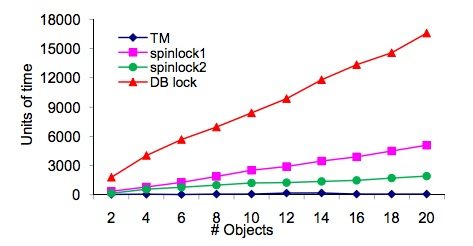
\includegraphics[width=0.3\textwidth]{figure/overhead.jpg}
  \caption{Overhead of CC approaches.}
  \label{fig:fcommon} 
\end{figure}

\bibliographystyle{plain}
\bibliography{ref}

\end{document}
% end doc
